\documentclass[conference]{IEEEtran}
% Add to the paper's preamble (or % Add to the paper's preamble (or % Add to the paper's preamble (or \input{tables/preamble} after \documentclass).
\usepackage{booktabs}          % \toprule \midrule \bottomrule
\usepackage[table]{xcolor}     % \cellcolor
\usepackage{graphicx}
\definecolor{bestbg}{RGB}{226,239,218}
% Best corrected model per engine and column (reviewer item #42: "color the best").
\newcommand{\best}[1]{\cellcolor{bestbg}\textbf{#1}}
 after \documentclass).
\usepackage{booktabs}          % \toprule \midrule \bottomrule
\usepackage[table]{xcolor}     % \cellcolor
\usepackage{graphicx}
\definecolor{bestbg}{RGB}{226,239,218}
% Best corrected model per engine and column (reviewer item #42: "color the best").
\newcommand{\best}[1]{\cellcolor{bestbg}\textbf{#1}}
 after \documentclass).
\usepackage{booktabs}          % \toprule \midrule \bottomrule
\usepackage[table]{xcolor}     % \cellcolor
\usepackage{graphicx}
\definecolor{bestbg}{RGB}{226,239,218}
% Best corrected model per engine and column (reviewer item #42: "color the best").
\newcommand{\best}[1]{\cellcolor{bestbg}\textbf{#1}}

\usepackage{amsmath}
\usepackage{cite}
\usepackage{url}

\begin{document}

\title{OCR-Engine-Agnostic Post-OCR Correction for Bengali Text using Small Language Models}

\author{\IEEEauthorblockN{Arifur Rahman}
\IEEEauthorblockA{ID: 20234103222\\
Department of Computer Science and Engineering\\
Bangladesh University of Business and Technology\\
Dhaka, Bangladesh\\
arifur.rahman.cs04@gmail.com}}

\maketitle

% =====================================================================
\begin{abstract}
Optical character recognition (OCR) for historical Bengali print is error-prone, and correcting its output with a small language model has been suggested as a low-cost remedy that needs no retraining. We test this suggestion on fifteen held-out pages of a British Library corpus of Bengali books. Two OCR engines (Tesseract and EasyOCR) produce the text, and four open models of at most two billion parameters (Gemma 2B, Llama 3.2 1B, TituLLMs 1B and BanglaT5) correct it zero-shot on a CPU with one fixed instruction (BanglaT5, which is not instruction-tuned, receives the text alone). In all eight engine-and-model combinations, correction raised both the character and the word error rate, and fifteen of the sixteen resulting increases (two metrics per combination) are significant under a paired bootstrap and a Holm-corrected Wilcoxon test. Gemma 2B produced the smallest CER increase, raising the character error rate from 0.364 to 0.583 on Tesseract output and from 0.297 to 0.517 on EasyOCR output. Correction altered between 76 and 99.5 percent of the words that the raw OCR had recognised correctly, while recovering at most 5.5 percent of those it had recognised incorrectly. The direction of the effect was the same for both engines. A length-based safeguard reduced the increase in error but never brought it below the uncorrected level. For the models, prompt and historical corpus tested here, zero-shot correction made Bengali OCR output worse; fine-tuning remains untested.
\end{abstract}

\begin{IEEEkeywords}
Bengali OCR, post-OCR correction, small language models, zero-shot prompting, low-resource NLP, negative results
\end{IEEEkeywords}

% =====================================================================
\section{Introduction}

Bengali ranks seventh among the world's languages by total speakers, with about 278 million~\cite{eberhard2025ethnologue}. OCR supports the conversion of printed Bengali records into searchable text, but published evaluations report high recognition error rates. In the evaluation reported with the bbOCR system, Tesseract reaches an average character error rate (CER) of 0.78 across Bengali document types, and the purpose-built bbOCR system reaches 0.59~\cite{zulkarnain2023bbocr}. A separate study puts Tesseract's character accuracy between 37 and 84 percent depending on the document type~\cite{rabby2024enhancement}. Several properties of the script complicate recognition. Consonants combine into conjunct glyphs, vowel signs attach before, after, above or below the consonant they modify, and many characters differ from their neighbours only in small strokes~\cite{rabby2024enhancement}. Historical books add worn type, uneven inking and ornate display lettering, and the corpora needed to train recognition models are small~\cite{zulkarnain2023bbocr}.

Language-model post-correction offers a way to process recognition errors without modifying the OCR engine. Small models may suit institutions with limited computing resources, including national archives, government offices and non-governmental organisations involved in Bengali digitisation. Their lower hardware requirements motivate evaluating them for resource-limited archives~\cite{vershinin2025lightweight}. A correction layer of this kind would also be engine-independent: it reads text, not images, so it could be attached to any OCR system without retraining.

Evidence on whether such a layer works is mixed outside English. Open-weight models improved OCR output in English but made Finnish worse~\cite{kanerva2025nofreelunches}. Zero-shot models, including a 70-billion-parameter one, increased the error rate once the input CER reached about 0.15~\cite{koynov2025opportunities}. For Hindi speech-recognition output, zero-shot language models raised the word error rate~\cite{kumar2026postasr}. For Bengali OCR we found no published study of language-model correction, and none that checks whether a correction layer behaves the same way across OCR engines. We evaluate the following research questions.
\begin{itemize}
\item \textbf{RQ1.} Can small open language models (at most two billion parameters), prompted zero-shot on a CPU, reduce the character and word error rates of Bengali OCR output?
\item \textbf{RQ2.} Is the effect of correction consistent across OCR engines when the correction step is not adapted to either engine?
\end{itemize}

Correction increased error rates for both engines. To examine this outcome, the study combines a held-out evaluation with analysis of changes to the recognised text. Its contributions are:
\begin{enumerate}
\item To our knowledge, it is the first evaluation of language-model post-correction for Bengali OCR, using two OCR engines and four models of at most two billion parameters.
\item It tests the result with paired statistics (a bootstrap and a Holm-corrected Wilcoxon test) on pages that were held out before any model was run.
\item It measures how the corrected text differs from the raw OCR: word-level counts of correct words broken and wrong words fixed, edit-operation profiles, script share, truncation, and dependence on page difficulty.
\item It evaluates a length-based fallback to raw OCR using thresholds from a published system.
\item It releases the code, the frozen page lists and the prompt, so the study can be repeated on free CPU-only infrastructure.
\end{enumerate}

% =====================================================================
\section{Related Work}

We review Bengali OCR systems, language-model post-correction, and Bengali language models and tokenisation. Related work on Indic text correction helps position the present evaluation.

\subsection{Bengali OCR systems}
Work on Bengali OCR has focused on recognition itself. bbOCR combines text detection, a purpose-built Bengali recognition model and layout reconstruction to convert whole documents into searchable text~\cite{zulkarnain2023bbocr}; it is compared only against Tesseract, with average text-level CER of 0.59 against 0.78. Rabby et al.\ train separate word-segmentation models for computer-composed, letterpress, typewritten and handwritten documents, and report Tesseract accuracy of 37 to 84 percent against 83 to 90 percent for their system~\cite{rabby2024enhancement}. At the level of single handwritten words, Safir et al.\ reach a CER of 0.091 and a WER of 0.273, using no surrounding context~\cite{safir2021endtoend}. These studies focus on recognition rather than a separate correction step for the remaining errors.

\subsection{Post-OCR correction with language models}
Task-specific fine-tuning has improved OCR correction in prior studies. Llama 2 tuned on short segments of 19th-century English newspapers reduced CER by 54.5 percent, against 23.3 percent for a fine-tuned BART~\cite{thomas2024leveraging}. Results without such tuning are less consistent. Kanerva et al.\ prompted open-weight models of 8 to 70 billion parameters on English and Finnish; most improved the English text, but every open model made the Finnish text worse, and only GPT-4o improved it~\cite{kanerva2025nofreelunches}. Koynov and Doan found that zero-shot GPT-4o-mini and Llama 3.3 70B cut CER by 48 to 58 percent on newspapers with an input CER of 0.07, but raised it by about 19 percent at 0.15 and, for Llama, by 41 percent on German text at 0.25~\cite{koynov2025opportunities}. Vershinin et al.\ ran four quantised 7 to 13 billion parameter models zero-shot on an English newspaper corpus (input CER 0.084); only one improved CER, and the others raised it, in one case five-fold~\cite{vershinin2025lightweight}. None of the instruction-tuned German models in another study reduced the average CER of a periodical, although the best one cut the word error rate by 22 percent; re-examining the outputs of an earlier study, the authors also found that inputs longer than about 400 characters degraded most~\cite{danilova2025german}.

The 2026 HIPE-OCRepair shared task compared zero-shot, fine-tuned and continued-pretraining systems of 8 to 24 billion parameters on English, French and German; the best system used continued pre-training and fine-tuning and finished ahead of the zero-shot systems, and over-correction of text that was already accurate was a recurring problem~\cite{ehrmann2026hipeocrepair}. In a study of Portuguese survey pages, a frontier model reduced CER from 11.7 to 4.7 percent~\cite{viana2026reframing}. Beshirov et al.\ improved historical Bulgarian, a non-Latin script, with a supervised two-stage system, but one that is specific to its engine and language~\cite{beshirov2025bulgarian}. Levchenko found that multimodal models transcribing 18th-century Russian text sometimes beat conventional OCR but inserted archaic characters from the wrong period~\cite{levchenko2025historical}. Witte's poster describes models that modernised historical language while appearing to correct it~\cite{witte2025postocr}.

\subsection{Bengali language models and tokenisation}
BanglaBERT is a Bengali encoder built for understanding tasks, not for rewriting text~\cite{bhattacharjee2022banglabert}. BanglaT5 is the corresponding sequence-to-sequence model for generation~\cite{bhattacharjee2023banglat5}. TituLLMs are Bengali-pretrained Llama 3.2 models at 1B and 3B parameters, trained on about 37 billion tokens with an extended tokenizer~\cite{nahin2025titullms}. BanglaLlama continues the pretraining of other Llama models and reports that Bangla and Hindi together make up less than 0.21 percent of Llama 2's pretraining tokens, against 89.7 percent for English~\cite{zehady2026banglallama}. Mahfuz et al.\ study whether dedicated Bengali models are needed at all, and find that inefficient tokenisation of Bengali raises computational cost and lowers generation quality~\cite{mahfuz2025toolate}. Related tokenisation disparities are reported across languages. Petrov et al.\ show that English-centric tokenizers need several times more tokens for the same text in many languages, with Bengali among them (roughly five to ten times the English count), while multilingual tokenizers such as XLM-R and M2M100 stay at about 1.4 to 1.6 times~\cite{petrov2023tokenizer}. Ahia et al.\ also report higher costs and poorer language-model performance for over-segmented languages~\cite{ahia2023cost}.

\subsection{Correction of Bengali and other Indic text}
The closest Bengali work corrects grammar, not OCR. Instruction-tuning raised Bangla grammar-correction scores by 3 to 7 points over the zero-shot setting, and humans still outperformed the models at correcting; the hardest categories for GPT-4o included mixing of the older literary register with the modern one~\cite{bhattacharyya2025banglagec}. For Hindi speech-recognition output, fine-tuned models of 0.3 to 0.58 billion parameters beat much larger language models, and zero-shot GPT-4o-mini raised the word error rate from 28.6 to 31.8 and from 18.0 to 25.1 percent. The authors trace this to over-correction, which grows with model size~\cite{kumar2026postasr}.

\subsection{Research gap}
Table~\ref{tab:literature} summarises the studies above. Among the work we reviewed, none evaluates post-OCR correction for Bengali, none tests models of at most two billion parameters on input with a CER above 0.3, and none compares one correction layer across OCR engines. These gaps motivate the choice of language, model scale and cross-engine evaluation.

% Literature comparison table (reviewer item #10: "Add tables if possible").
% Every cell was checked against the paper itself; see reviewer-feedback/paper-reviews.md.
% Keys refer to paper/references.bib.
\begin{table*}[t]
\centering
\caption{Language-Model Correction of Recognition Output: Prior Work and This Study}
\label{tab:literature}
\setlength{\tabcolsep}{3.5pt}
\footnotesize
\begin{tabular}{p{2.6cm}p{1.2cm}p{1.6cm}p{3.3cm}p{1.6cm}p{1.6cm}p{3.6cm}}
\toprule
Study & Language & Task & Models (size) & Setting & Input error & Did correction help? \\
\midrule
Thomas et al.~\cite{thomas2024leveraging} & English & post-OCR & Llama 2 (7B, 13B); BART & fine-tuned & CER 0.08 & Yes: CER $-$54.5\% (13B) \\
Danilova \& Aangenendt~\cite{danilova2025german} & German & post-OCR & Llama 2 13B, Mistral 7B; BART & fine-tuned & CER 0.02 & No CER gain on average; WER $-$22\% (best) \\
Kanerva et al.~\cite{kanerva2025nofreelunches} & English, Finnish & post-OCR & open models 8B--70B; GPT-4o & zero-shot & CER 0.07 / 0.09 & English: 6 of 7 models; Finnish: only GPT-4o \\
Koynov \& Doan~\cite{koynov2025opportunities} & English, German & post-OCR & GPT-4o-mini; Llama 3.3 70B & zero-shot (+ fine-tuned) & CER 0.07--0.25 & Yes at CER 0.07; worse at CER $\geq$0.15 \\
Vershinin et al.~\cite{vershinin2025lightweight} & English & post-OCR & 7B--13B, 4-bit quantized & zero-shot & CER 0.08 & 1 of 4 models improved CER \\
Beshirov et al.~\cite{beshirov2025bulgarian} & Bulgarian & post-OCR & BERT detector + LSTM corrector & supervised & --- & Yes \\
Ehrmann et al.~\cite{ehrmann2026hipeocrepair} & English, French, German & post-OCR & 8B--24B & zero-shot; fine-tuned & CER 0.004--0.057 & Fine-tuned: yes; zero-shot: mixed (worse than raw OCR on French) \\
Viana~\cite{viana2026reframing} & Portuguese & post-OCR & GPT-5.5 (frontier) & zero-shot & CER 0.12 & Yes: CER $-$60\% \\
Bhattacharyya \& Bhattacharya~\cite{bhattacharyya2025banglagec} & Bengali & grammar correction & 1.1B--8B; GPT-4o & zero-shot; fine-tuned & clean modern text & Fine-tuned 3--7 points above zero-shot \\
Kumar et al.~\cite{kumar2026postasr} & Hindi & post-ASR & Llama 1B--70B, GPT-4o-mini; mT5, ByT5 (0.3--0.58B) & zero-shot; fine-tuned & WER 0.18--0.29 & Zero-shot: worse; fine-tuned small models: yes \\
\midrule
\textbf{This study} & \textbf{Bengali} & \textbf{post-OCR} & \textbf{0.25B--2B} & \textbf{zero-shot, CPU} & \textbf{CER 0.30--0.36} & \textbf{No: worse in 8/8 engine-model combinations} \\
\bottomrule
\end{tabular}
\end{table*}


% =====================================================================
\section{Methodology}

The evaluation compares raw and corrected OCR text against the same ground truth. The following subsections specify the dataset, OCR engines, correction configuration, model selection and scoring protocol.

\subsection{Overview}
Figure~\ref{fig:method} shows the pipeline. Two OCR engines read each page image. Their raw text is split into chunks and passed to a correction model, and both the raw and the corrected text are scored against a manual transcription. OCR and correction are separate stages, so the same correction step can be attached to the output of any engine. No model is trained or fine-tuned, and every model is used as released.

\begin{figure*}[t]
\centering
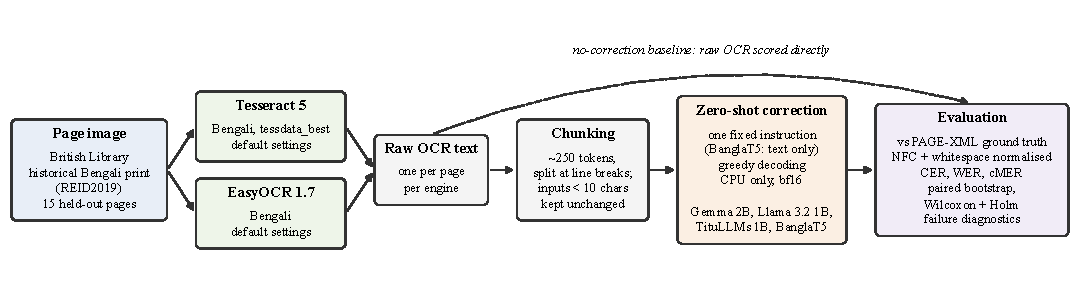
\includegraphics[width=\textwidth]{figures/fig_method.pdf}
\caption{Pipeline of the study. Each page image is read by two OCR engines. The raw text is chunked and corrected zero-shot by one of four models, and both raw and corrected text are scored against the ground truth. The dashed arrow marks the uncorrected baseline: raw OCR scored directly.}
\label{fig:method}
\end{figure*}

\subsection{Dataset}
We use the ground-truth transcriptions released with the ICDAR 2019 Competition on Recognition of Early Indian Printed Documents (REID2019)~\cite{clausner2019reid}, produced by the British Library's Two Centuries of Indian Print project with the PRImA Research Lab and Jadavpur University~\cite{britishlibrary2019bengaligt}. The source volumes are Bengali books printed between 1713 and 1914. The digitised images are out of copyright and the transcriptions are in the public domain.

The release contains 81 page images with PAGE-XML annotations. Twenty-nine of them (36\%) have text regions marked but no transcribed text, so no error rate can be computed, and they are excluded; 52 pages remain. We drop the two pages with the thinnest transcriptions, measured by the share of text regions that actually contain text, which leaves a pool of 50 pages. The pool is split into 10 development pages, used only to debug the pipeline, and 40 evaluation pages. The split was frozen in saved page-identifier lists and committed to version control before any correction model was run. From the 40 evaluation pages we scored a random sample of 15 (seed 403) through the full engine-by-model sweep, the largest number that the CPU-only budget allowed. All reported results come from these 15 pages, and no development page contributes to any reported figure (Fig.~\ref{fig:dataset}). The scored pages have a median ground-truth length of 577 characters; several are verse or title pages in ornate display type.

\begin{figure*}[t]
\centering
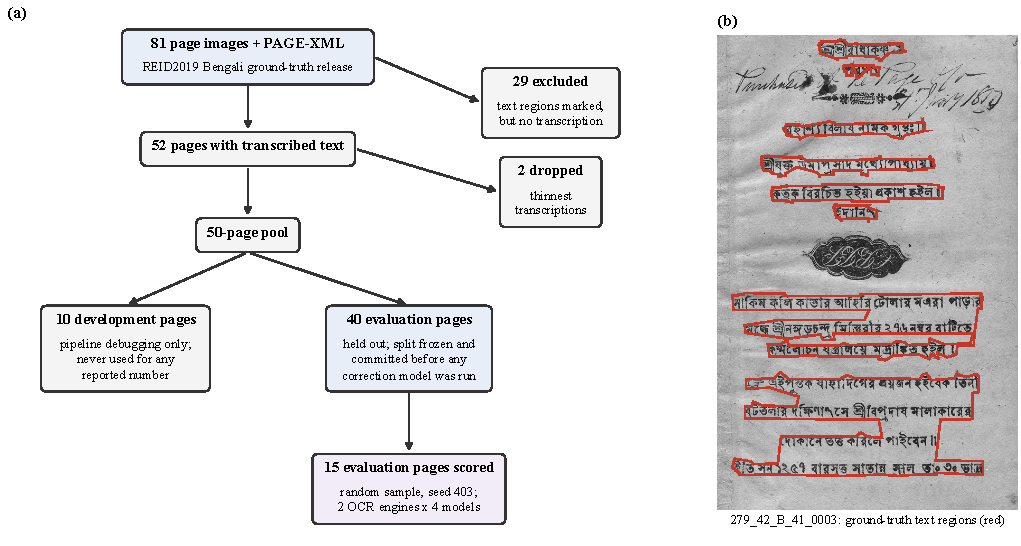
\includegraphics[width=\textwidth]{figures/fig_dataset.pdf}
\caption{Dataset. (a) How the 81 pages of the release become the 15 scored pages. (b) A sample evaluation page, with the ground-truth text regions outlined in red.}
\label{fig:dataset}
\end{figure*}

\subsection{Baseline OCR}
Two open-source engines produce the noisy text: Tesseract~\cite{smith2007tesseract} with the Bengali \texttt{tessdata\_best} model, and EasyOCR~\cite{jaidedai2024easyocr} with Bengali enabled. Each engine runs on every evaluation image with default settings and produces one hypothesis per page. Two engines with different error profiles let us test whether correction behaves differently depending on which engine produced its input.

\subsection{Correction layer}
\textbf{Zero-shot.} Here, zero-shot evaluation uses no worked correction examples or task-specific weight updates. The decoder models receive an instruction and the OCR text; BanglaT5 receives the text alone, as detailed below. We chose this setting because we know of no large public set of Bengali OCR error pairs for training, and because it avoids the cost of task-specific training.

\textbf{Prompt.} The four decoder models receive the same instruction, through each model's chat template:
\begin{quote}
\small\itshape
The following text was produced by OCR on a historical Bengali document and may contain recognition errors. Correct the OCR errors and output only the corrected Bengali text, with no explanation, preamble, or additional commentary.
\end{quote}
The OCR text follows the instruction. BanglaT5 is not instruction-tuned and has no chat template, so it receives the OCR text alone and is run as a text-to-text model. The prompt was fixed in advance and never revised in response to model output, so differences between conditions are not attributable to prompt revisions.

\textbf{Chunking.} Following Kanerva et al.~\cite{kanerva2025nofreelunches}, each page is divided into chunks of about 250 tokens of the model's own tokenizer before correction. Chunks are formed by grouping complete lines, so no chunk boundary falls inside a line. A page whose raw OCR is shorter than ten characters would be left unchanged, since the model would have almost nothing to work from; no evaluation page triggered this rule.

\textbf{Decoding.} Decoding is greedy, so output is deterministic. The maximum number of new tokens is $\min(512,\max(64,1.5n))$, where $n$ is the token length of the input chunk, and an output that reaches this limit is counted as truncated. No other constraint is applied. Our first runs also used a repetition penalty of 1.3 and banned repeated four-grams. We added these two settings after a development-set run in which one model repeated a single phrase until it reached the length limit, so, unlike the prompt, they were chosen after seeing model output. In the generation function of the Transformers library~\cite{wolf2020transformers}, both settings act on the whole token sequence, which for a decoder-only model includes the prompt and therefore the OCR text being corrected. They penalise every token the model copies from its input and forbid it from reproducing any four-token run of that input. Because correction consists mostly of copying, we use the setting without them as the main condition and report the original setting as a decoding ablation (Section~\ref{sec:decoding}).

\subsection{Choice of models}
We evaluate five models, all small enough for CPU inference. The parameter counts below are computed from each checkpoint's configuration, with tied input and output embeddings counted once.
\begin{itemize}
\item \emph{Llama 3.2 1B} (1.24B parameters)~\cite{meta2024llama32} and \emph{Gemma 2B} (2.51B)~\cite{gemma2024} are open instruction-tuned models that represent general-purpose multilingual models. Bengali is a very small share of their pretraining data~\cite{zehady2026banglallama}.
\item \emph{Qwen3 1.7B} (1.72B)~\cite{yang2025qwen3} is a general-purpose model released in 2025, added in revision to test whether a more recent model behaves differently. It can produce a reasoning trace before its answer; we disable this through its chat template, so it answers directly.
\item \emph{TituLLMs 1B}~\cite{nahin2025titullms} is a Bengali-pretrained model built on Llama 3.2 1B with an extended tokenizer. It has the same size and base architecture as Llama 3.2 1B, which supports a comparison at a similar parameter count. The extended tokenizer and possible differences in other training details prevent this comparison from isolating the effect of Bengali pretraining.
\item \emph{BanglaT5} (about 248M parameters)~\cite{bhattacharjee2023banglat5} is a Bengali sequence-to-sequence model. Its text-to-text architecture provides a sequence-to-sequence baseline for correction. It is used as released, without fine-tuning.
\end{itemize}
Phi-3 Mini (3.8B) was implemented but not run to completion: the evaluated models took between about two and fourteen minutes per page on average, and up to 30 minutes for one page, and a 3.8-billion-parameter model did not fit the available budget. BanglaBERT~\cite{bhattacharjee2022banglabert} was not considered because it is an encoder and cannot generate corrected text. All models are loaded with the Transformers library~\cite{wolf2020transformers} in bfloat16.

\subsection{Deployment setting}
All models run in CPU-only mode on a free Google Colab runtime. This approximates the setting that motivates the work: institutions in Bangladesh that process large volumes of Bengali documents and typically lack GPU infrastructure. No paid API is used at any stage.

\subsection{Evaluation protocol}
\textbf{Normalisation and metrics.} Before scoring, reference and hypothesis are normalised to Unicode NFC and runs of whitespace are collapsed, because Bengali conjuncts and vowel signs can be encoded as different codepoint sequences that look identical. CER and WER are computed with jiwer~\cite{vaessen2022jiwer} for each page and averaged over pages, so every page counts equally regardless of its length. CER is unbounded: an output with more erroneous characters than the reference has characters scores above 1. We therefore also report the character match error rate, $\mathrm{cMER}=(S+D+I)/(H+S+D+I)$, which counts insertions in the denominator and is bounded in $[0,1]$~\cite{ehrmann2026hipeocrepair}. Here $H$, $S$, $D$ and $I$ are the numbers of matched, substituted, deleted and inserted characters.

\textbf{Statistical testing.} For each engine and model, the unit of analysis is the per-page difference between the corrected and the uncorrected error rate. We report the mean difference with a 95\% percentile interval from a paired bootstrap of the 15 pages (10{,}000 resamples, seed 403). We also run a two-sided Wilcoxon signed-rank test~\cite{wilcoxon1945} on the same differences and adjust the $p$-values with the Holm procedure~\cite{holm1979} over the 20 CER and WER tests, which follows the reporting of Viana~\cite{viana2026reframing}.

\textbf{Validation.} The held-out split was frozen before any model ran, and development pages are never scored. We used one fixed held-out evaluation set and did not perform cross-validation. No model was trained, and deterministic decoding was not repeated with different seeds. Each page is paired with its own uncorrected text.

\textbf{Word-level and edit analysis.} To see what correction changes, we align the ground-truth words with the raw OCR and with the corrected output. A ground-truth word that the raw OCR matched exactly and the output does not is a \emph{broken} word; a word the raw OCR missed and the output matches is a \emph{fixed} word~\cite{kumar2026postasr}. The \emph{change ratio} is the CER of the output measured against the raw OCR, divided by the CER of the raw OCR against the ground truth~\cite{koynov2025opportunities}; a ratio above 1 means the model changed more than there was to repair. \emph{Invented runs} are runs of at least six characters that the output contains and the raw OCR does not~\cite{koynov2025opportunities}. We also report output length relative to the reference, the share of Bengali, Latin and other characters, ground-truth word retention, and the truncation rate.

\textbf{Safeguard.} As a post-hoc check, we replace a model's output by the raw OCR whenever its length falls outside 0.35 to 2.8 times the input length. These thresholds are taken from a zero-shot system in the HIPE-OCRepair task~\cite{ehrmann2026hipeocrepair} and are not tuned on our pages.

\textbf{Deviation from the intended protocol.} Kanerva et al.\ strip leading and trailing text that does not align with the input, such as explanatory preambles~\cite{kanerva2025nofreelunches}. We specified this step but did not implement it, so all scores use unfiltered model output and any preamble or commentary counts as error. Section~\ref{sec:discussion} discusses what this means.

\subsection{Reproducibility}
The page lists, the correction prompt, and the OCR, correction, scoring and statistics code are public~\cite{rahman2026repo}, with the frozen split committed before any model was run. Nothing is trained and no paid service is used, so the study can be repeated end to end on a free CPU-only runtime.

% =====================================================================
\section{Results}

Results compare each corrected output with its corresponding raw OCR baseline. Unless stated otherwise, they use plain greedy decoding (Section~\ref{sec:decoding} reports the original decoding setting). We also examine differences between engines, variation across pages and results under the bounded error metric.

\subsection{Baseline OCR performance}
Table~\ref{tab:baseline} gives the error rates of the raw OCR text before any correction. EasyOCR is better than Tesseract on all three metrics (CER 0.297 against 0.364). This agrees with the high Tesseract error rates on Bengali reported in earlier work~\cite{zulkarnain2023bbocr,rabby2024enhancement}. We did not find a published comparison of the two engines on historical Bengali print. Both baselines are high in absolute terms: EasyOCR, the better engine, has a CER of 0.297 and a WER of 0.719.

\begin{table}[t]
\centering
\caption{Uncorrected OCR Baselines (15 Evaluation Pages)}
\label{tab:baseline}
\begin{tabular}{lccc}
\toprule
Engine & CER & WER & cMER \\
\midrule
Tesseract & 0.364 & 0.810 & 0.336 \\
EasyOCR & 0.297 & 0.719 & 0.257 \\
\bottomrule
\end{tabular}
\end{table}


\subsection{Effect of correction}
Table~\ref{tab:matrix} gives the full evaluation matrix, and Figs.~\ref{fig:cer} and~\ref{fig:ci} show the same result graphically. No model lowered the mean error rate significantly for either engine. Of the 20 CER and WER comparisons, six are significant after Holm correction, and all six are increases: BanglaT5 on CER and TituLLMs on CER and WER, for both engines. TituLLMs on EasyOCR output has the largest increase, from a CER of 0.297 to 1.029.

The three general-purpose models stay close to the baseline. Gemma 2B ends at a CER of 0.360 on Tesseract output and 0.301 on EasyOCR output, against baselines of 0.364 and 0.297, and Qwen3 1.7B at 0.380 and 0.310; none of these differences is significant, and every bootstrap interval spans zero. Llama 3.2 1B raises CER to 0.430 and 0.337. Its bootstrap intervals lie above zero ($[+0.018,+0.116]$ and $[+0.005,+0.082]$), but the Holm-corrected Wilcoxon test does not reject the null hypothesis ($p=0.16$ and $p=0.36$). Its WER does not change significantly.

\begin{table*}[t]
\centering
\caption{Full Evaluation Matrix: 15 Pages, 2 Engines, 5 Models}
\label{tab:matrix}
\setlength{\tabcolsep}{4pt}
\footnotesize
\begin{tabular}{llccccccc}
\toprule
Engine & Model & CER & $\Delta$CER [95\% CI] & $p_{\mathrm{Holm}}$ & WER & $\Delta$WER [95\% CI] & $p_{\mathrm{Holm}}$ & Trunc. \\
\midrule
Tesseract & (no correction) & 0.364 & --- & --- & 0.810 & --- & --- & --- \\
Tesseract & Gemma 2B & \best{0.360} & \best{-0.004} [-0.013, +0.002] & 1.00\textsuperscript{ns} & 0.787 & -0.023 [-0.062, +0.001] & 1.00\textsuperscript{ns} & \best{0\%} \\
Tesseract & Qwen3 1.7B & 0.380 & +0.016 [-0.007, +0.047] & 1.00\textsuperscript{ns} & 0.796 & -0.014 [-0.036, +0.004] & 1.00\textsuperscript{ns} & 7\% \\
Tesseract & Llama 3.2 1B & 0.430 & +0.066 [+0.018, +0.116] & 0.16\textsuperscript{ns} & \best{0.776} & \best{-0.034} [-0.193, +0.120] & 1.00\textsuperscript{ns} & 7\% \\
Tesseract & BanglaT5 & 0.900 & +0.536 [+0.409, +0.650] & 0.001 & 0.983 & +0.173 [-0.105, +0.402] & 1.00\textsuperscript{ns} & 13\% \\
Tesseract & TituLLMs 1B & 0.929 & +0.565 [+0.432, +0.698] & 0.001 & 1.448 & +0.638 [+0.426, +0.848] & 0.003 & 100\% \\
\midrule
EasyOCR & (no correction) & 0.297 & --- & --- & 0.719 & --- & --- & --- \\
EasyOCR & Gemma 2B & \best{0.301} & \best{+0.004} [-0.014, +0.017] & 1.00\textsuperscript{ns} & 0.728 & +0.009 [-0.007, +0.025] & 1.00\textsuperscript{ns} & \best{0\%} \\
EasyOCR & Qwen3 1.7B & 0.310 & +0.013 [-0.005, +0.035] & 1.00\textsuperscript{ns} & \best{0.712} & \best{-0.007} [-0.039, +0.028] & 1.00\textsuperscript{ns} & 7\% \\
EasyOCR & Llama 3.2 1B & 0.337 & +0.040 [+0.005, +0.082] & 0.36\textsuperscript{ns} & 0.718 & -0.001 [-0.047, +0.041] & 1.00\textsuperscript{ns} & 7\% \\
EasyOCR & BanglaT5 & 0.837 & +0.540 [+0.438, +0.628] & 0.001 & 1.067 & +0.348 [+0.129, +0.562] & 0.14\textsuperscript{ns} & 13\% \\
EasyOCR & TituLLMs 1B & 1.029 & +0.732 [+0.614, +0.842] & 0.001 & 1.457 & +0.738 [+0.535, +0.939] & 0.001 & 100\% \\
\bottomrule
\end{tabular}
\par\smallskip
\begin{minipage}{\linewidth}\footnotesize $\Delta$ = corrected $-$ uncorrected (positive = worse). CI: paired bootstrap, 10{,}000 resamples, seed 403. $p_{\mathrm{Holm}}$: two-sided Wilcoxon signed-rank, Holm-corrected over the 20 tests. ns: not significant. Trunc.: pages whose output hit the token cap. \colorbox{bestbg}{\textbf{Shaded}}: best corrected model per engine.\end{minipage}
\end{table*}


\begin{figure}[t]
\centering
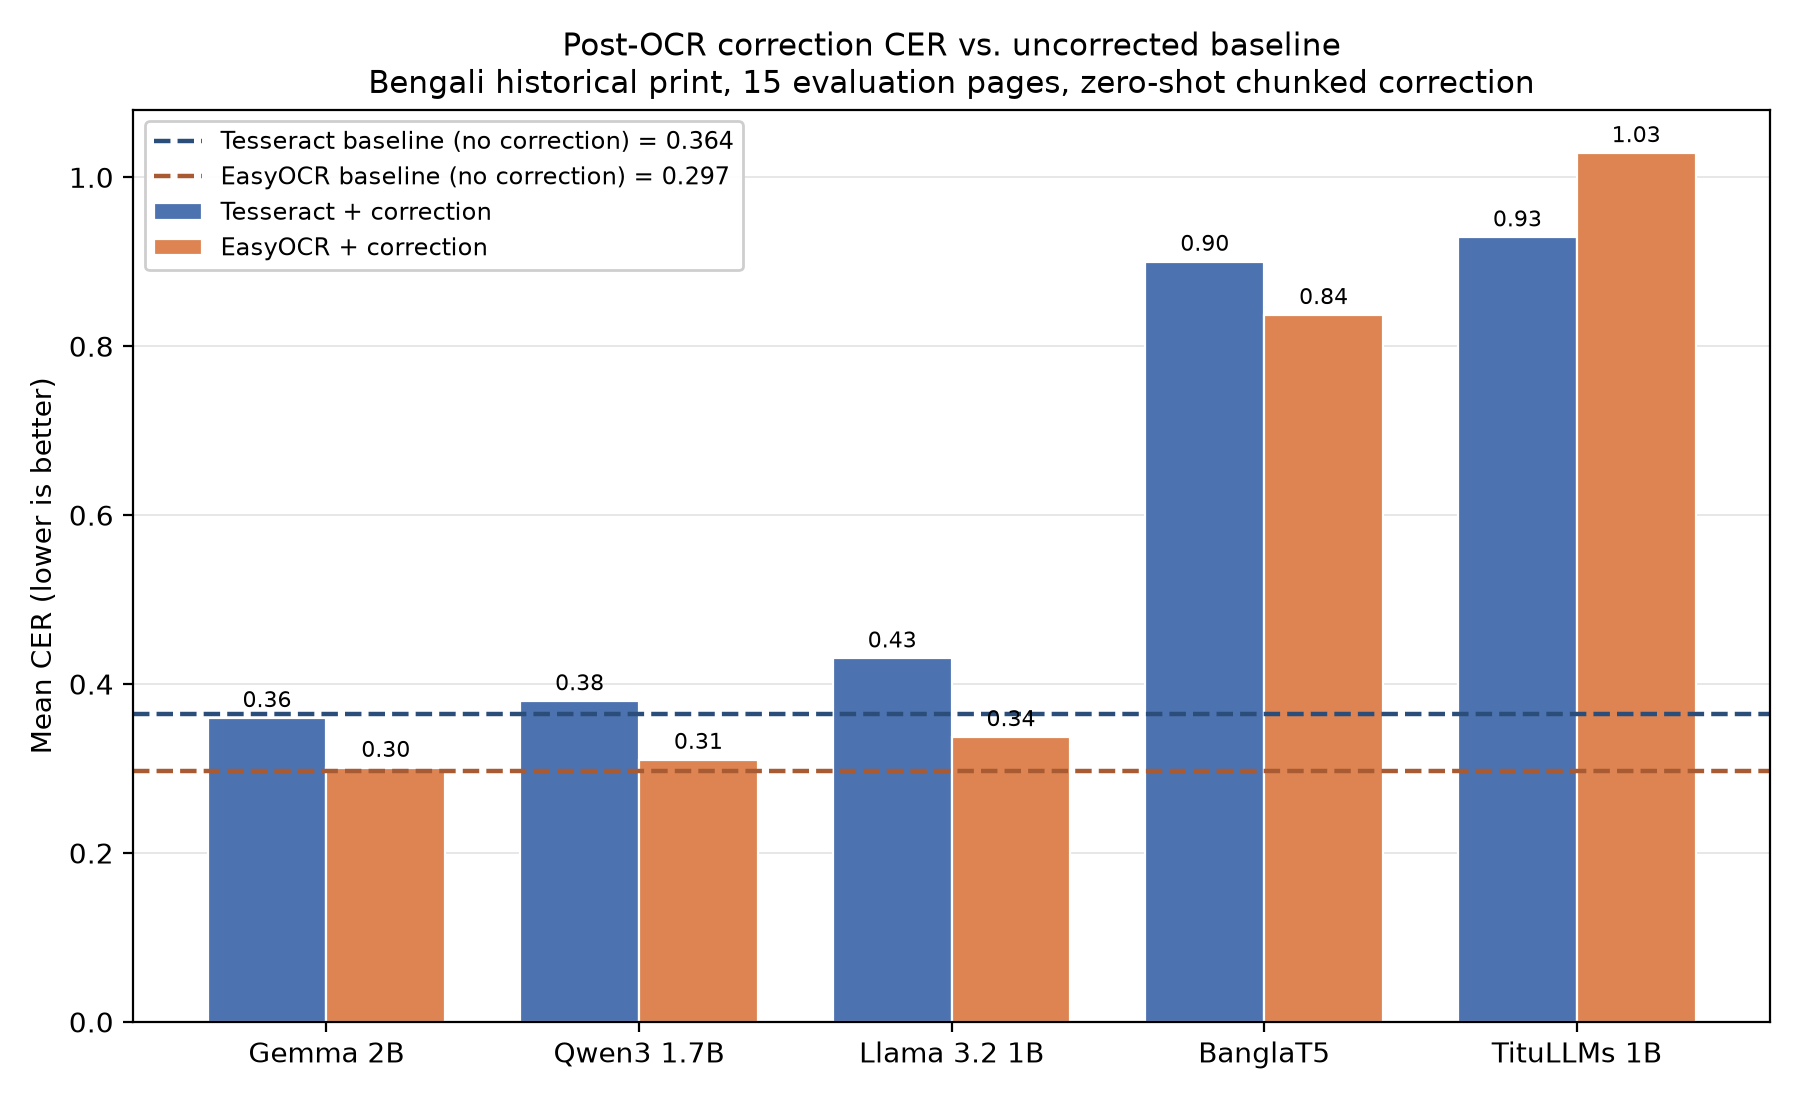
\includegraphics[width=\columnwidth]{figures/fig1_cer_by_model.png}
\caption{Mean CER over the 15 pages after correction, by model and OCR engine. The dashed lines mark the uncorrected baselines (Tesseract 0.364, EasyOCR 0.297).}
\label{fig:cer}
\end{figure}

\begin{figure}[t]
\centering
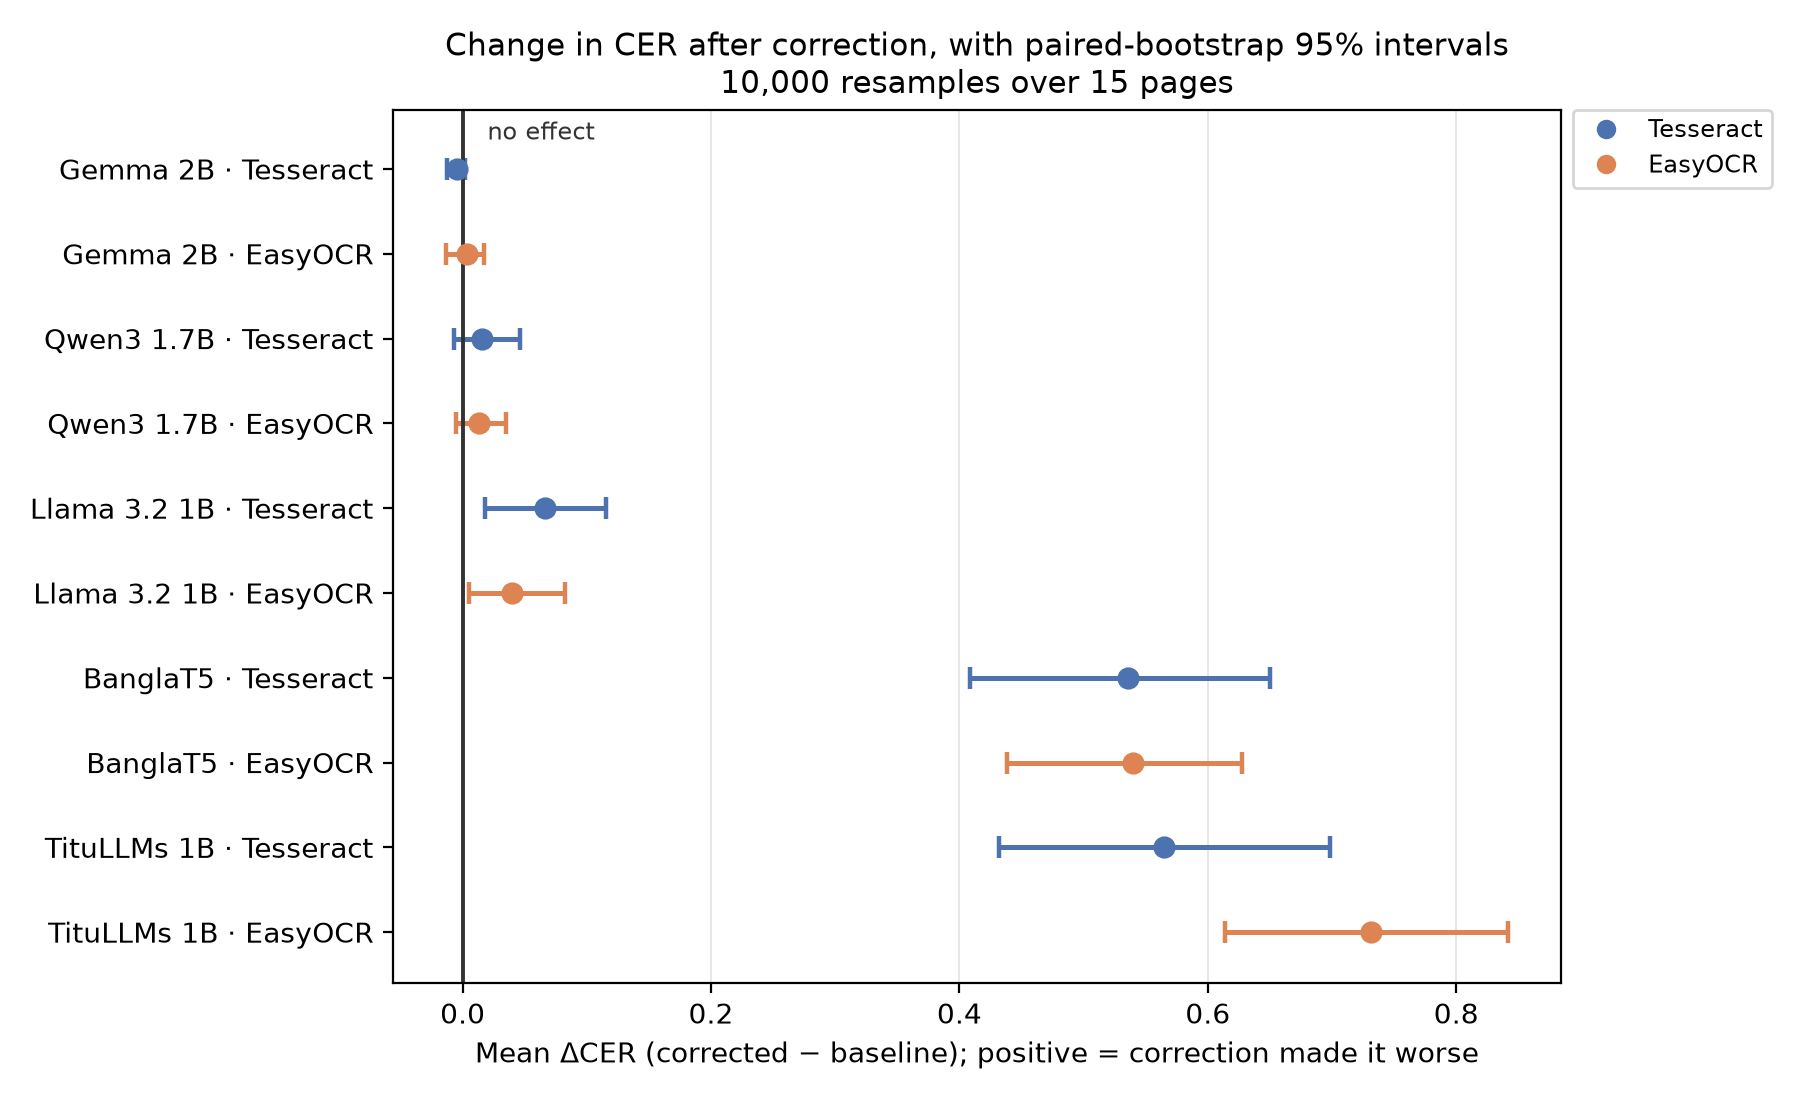
\includegraphics[width=\columnwidth]{figures/fig2_bootstrap_ci.png}
\caption{Mean change in CER (corrected minus uncorrected) for each model and engine, with 95\% paired-bootstrap intervals over the 15 pages. A value above zero means correction made the text worse.}
\label{fig:ci}
\end{figure}

\subsection{Effect of the decoding setting}
\label{sec:decoding}
Table~\ref{tab:decoding} compares the original decoding setting, with the repetition penalty and the four-gram ban, against plain greedy decoding. For the three decoder-only models that were run in both settings, removing the two constraints lowered CER significantly for both engines: by 0.22 for Gemma 2B, by 0.41 and 0.56 for Llama 3.2 1B, and by 1.07 and 1.56 for TituLLMs. Under the original setting Gemma 2B raised CER from 0.364 to 0.583 and from 0.297 to 0.517; under plain decoding it returns the input almost unchanged, with a median CER of 0.012 and 0.005 between its output and its own input. Most of the error increase that the original setting produced for these models is therefore attributable to the decoding constraints and not to the models' corrections. BanglaT5, an encoder-decoder model whose decoder does not see the input tokens as its own history, changed by 0.011 and 0.020. Qwen3 1.7B was added after this comparison and was run with plain decoding only.

\begin{table*}[t]
\centering
\caption{Decoding Ablation: Repetition Guards versus Plain Greedy Decoding (Mean CER)}
\label{tab:decoding}
\setlength{\tabcolsep}{4pt}
\footnotesize
\begin{tabular}{llccccc}
\toprule
Engine & Model & Raw OCR & Guarded & Plain & Plain $-$ guarded [95\% CI] & \shortstack{Plain output vs.\\its input (median CER)} \\
\midrule
Tesseract & Gemma 2B & 0.364 & 0.583 & 0.360 & -0.224 [-0.295, -0.155] & 0.012 \\
Tesseract & Llama 3.2 1B & 0.364 & 0.844 & 0.430 & -0.413 [-0.510, -0.308] & 0.163 \\
Tesseract & BanglaT5 & 0.364 & 0.889 & 0.900 & +0.011 [-0.007, +0.028] & 0.875 \\
Tesseract & TituLLMs 1B & 0.364 & 1.996 & 0.929 & -1.067 [-1.444, -0.685] & 0.956 \\
\midrule
EasyOCR & Gemma 2B & 0.297 & 0.517 & 0.301 & -0.216 [-0.300, -0.154] & 0.005 \\
EasyOCR & Llama 3.2 1B & 0.297 & 0.897 & 0.337 & -0.560 [-0.694, -0.434] & 0.065 \\
EasyOCR & BanglaT5 & 0.297 & 0.817 & 0.837 & +0.020 [+0.005, +0.037] & 0.836 \\
EasyOCR & TituLLMs 1B & 0.297 & 2.588 & 1.029 & -1.559 [-2.161, -0.958] & 0.957 \\
\bottomrule
\end{tabular}
\par\smallskip
\begin{minipage}{\linewidth}\footnotesize Guarded: \texttt{repetition\_penalty}=1.3 and \texttt{no\_repeat\_ngram\_size}=4, as in the original runs; for decoder-only models both also act on the prompt, so they penalise copying the OCR text. Plain: neither; greedy decoding with only the length cap. CI: paired bootstrap, 10{,}000 resamples, seed 403. Last column: CER of the plain output against its own OCR input (near 0 = the model returned its input almost unchanged).\end{minipage}
\end{table*}


\subsection{The engine-agnostic question}
The ranking of the models is the same for both engines: Gemma 2B, Qwen3 1.7B, Llama 3.2 1B, BanglaT5 and TituLLMs, from lowest to highest corrected CER. The changes in CER agree closely for Gemma 2B ($-0.004$ against $+0.004$), Qwen3 1.7B ($+0.016$ against $+0.013$) and BanglaT5 ($+0.536$ against $+0.540$), and less closely for Llama 3.2 1B ($+0.066$ against $+0.040$) and TituLLMs ($+0.565$ against $+0.732$), Tesseract first. These are descriptive comparisons; they do not establish equivalence in effect size.

\subsection{Per-page analysis}
Across the 150 page-level cells (15 pages, 5 models, 2 engines), correction lowered CER in 27: 14 for Qwen3 1.7B, 9 for Gemma 2B and 4 for Llama 3.2 1B. BanglaT5 and TituLLMs lowered CER on no page. Figure~\ref{fig:perpage} shows that the general-purpose models track the baseline closely, while BanglaT5 and TituLLMs stay near or above a CER of 0.8 on most pages.

For the models that changed the text substantially, the increase depends on page difficulty. When the pages are split into thirds by baseline CER, BanglaT5 and TituLLMs have their smallest increase on the hardest third for both engines; for TituLLMs on Tesseract output, for example, the increase is $+0.85$ on the easiest third and $+0.26$ on the hardest. Llama 3.2 1B shows the same pattern on a smaller scale ($+0.10$ on the easiest third of Tesseract pages and $-0.002$ on the hardest). The changes for Gemma 2B and Qwen3 1.7B stay within 0.03 of zero in every third. The HIPE-OCRepair task also reports over-correction of low-noise input~\cite{ehrmann2026hipeocrepair}.

\begin{figure*}[t]
\centering
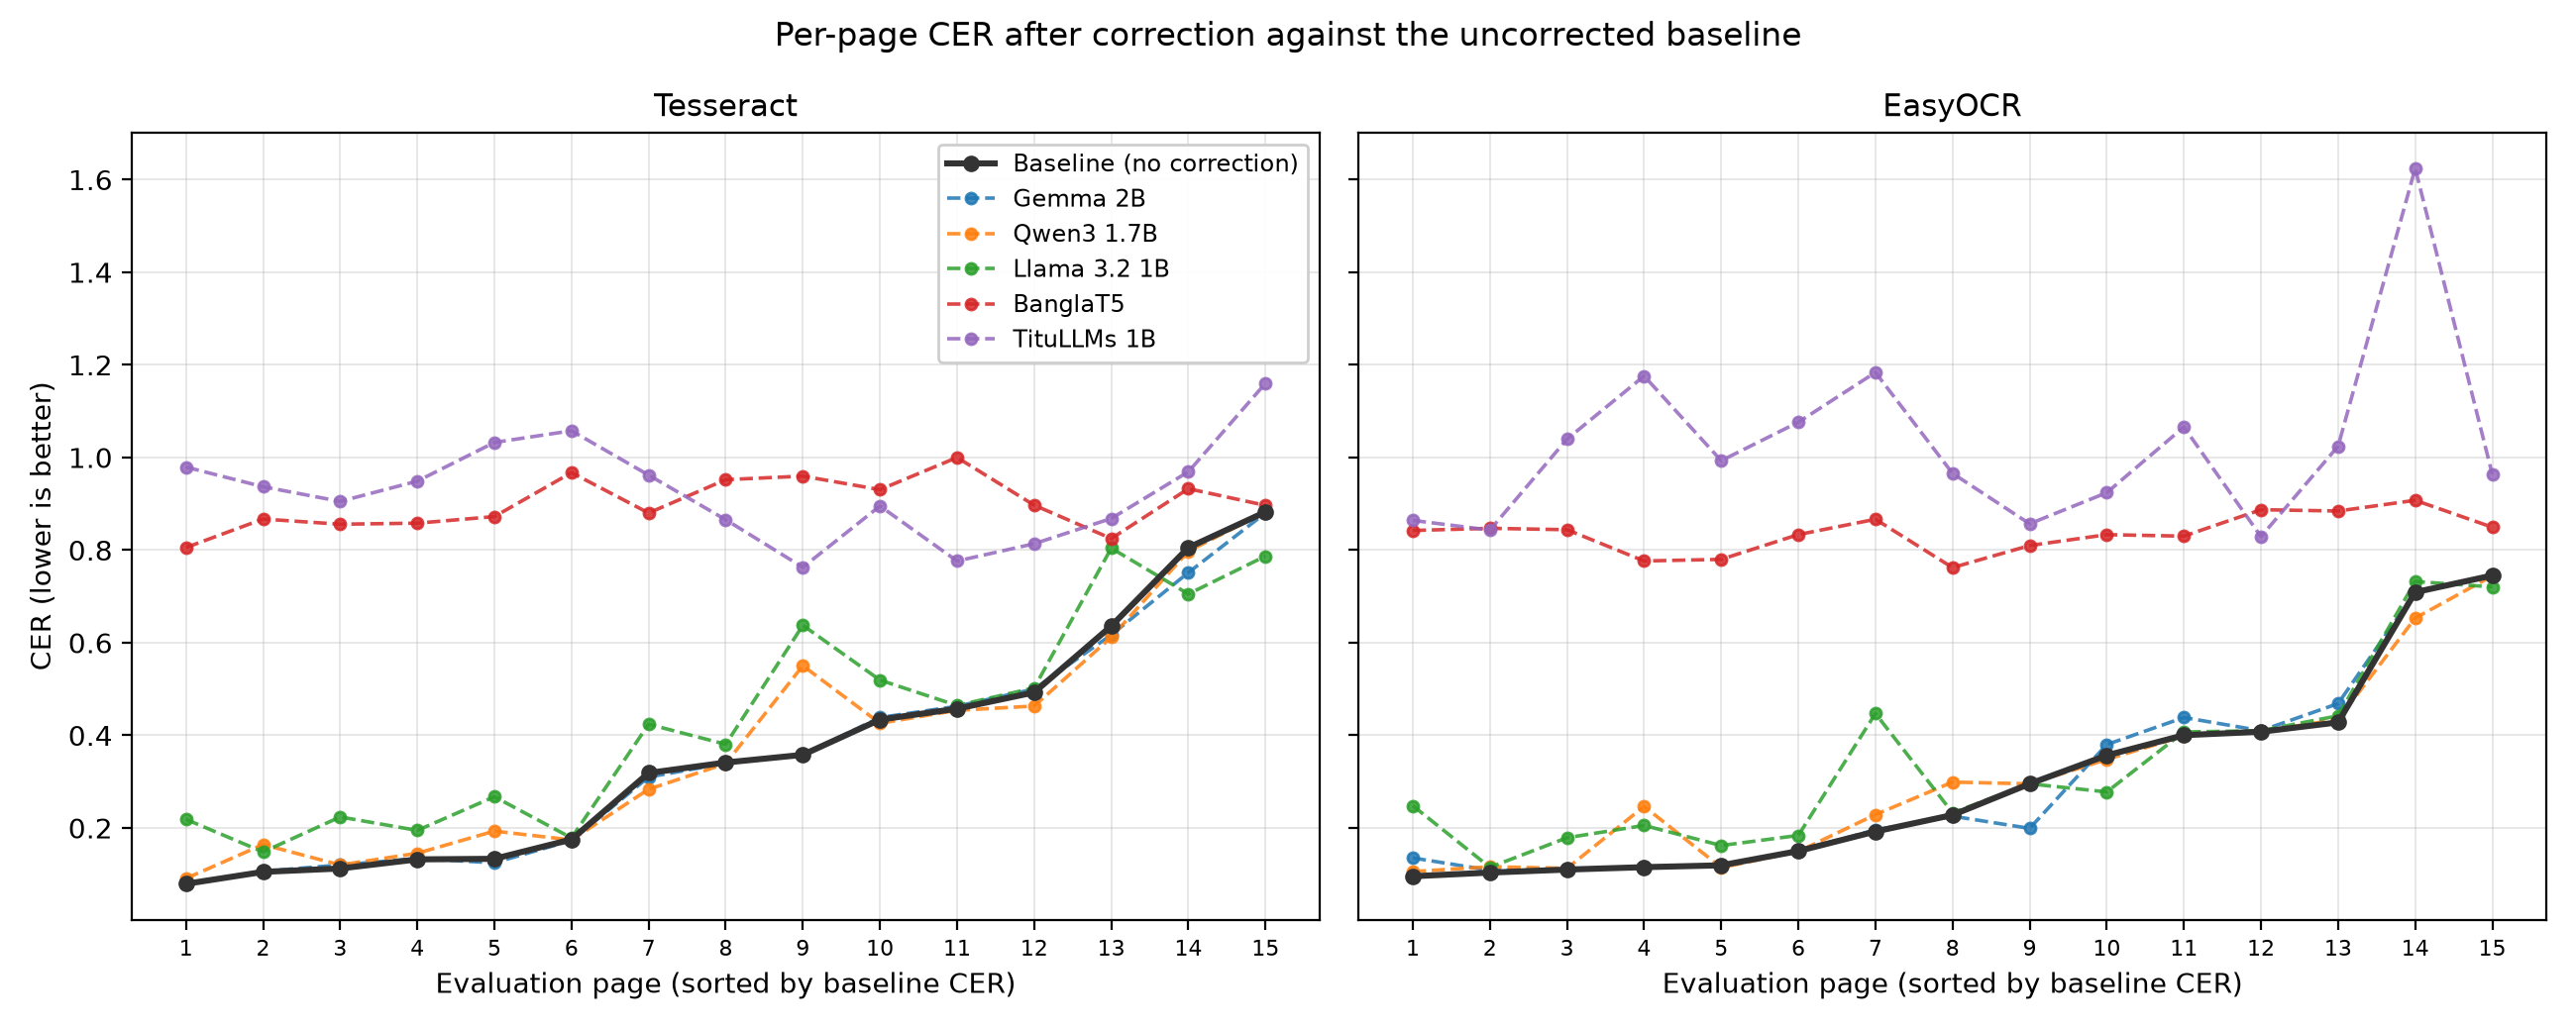
\includegraphics[width=0.9\textwidth]{figures/fig3_per_page.png}
\caption{CER per evaluation page, with pages sorted from easiest to hardest by baseline CER, for Tesseract (left) and EasyOCR (right). The solid black line is the uncorrected baseline; each dashed line is one correction model.}
\label{fig:perpage}
\end{figure*}

\subsection{Bounded error rate}
Because CER can exceed 1, we repeated the analysis with cMER (Table~\ref{tab:damage}). The baseline cMER is 0.336 for Tesseract and 0.257 for EasyOCR. Six of the ten cMER tests are significant after Holm correction, all of them increases: Llama 3.2 1B (0.416 and 0.306), BanglaT5 (0.900 and 0.835) and TituLLMs (0.703 and 0.669). Gemma 2B (0.336 and 0.262) and Qwen3 1.7B (0.353 and 0.272) do not differ significantly from the baseline. The two metrics therefore agree except for Llama 3.2 1B, whose CER increase is not significant after Holm correction but whose cMER increase is.

% =====================================================================
\section{Failure Analysis}

To characterize what correction changed, we examine word retention, edit operations and truncation. We then evaluate whether a length-based fallback reduces the error increases.

\subsection{Word retention and word-level changes}
Table~\ref{tab:diagnostics} reports how many ground-truth words each output retains. Raw Tesseract output keeps 46\% of the distinct ground-truth words and raw EasyOCR output 55\%. Pooled over both engines, Gemma 2B and Qwen3 1.7B keep 49\% and 50\%, Llama 3.2 1B 45\%, TituLLMs 17\% and BanglaT5 2\%. The word-level counts in Table~\ref{tab:damage} separate correct words that were changed from wrong words that were fixed. Gemma 2B broke 1\% and 3\% of the words the raw OCR had right and fixed almost none of those it had wrong (0.4\% and 0.0\%). Qwen3 1.7B is the only model whose repairs come close to its damage: on Tesseract text it fixed 47 wrong words and broke 62 correct ones, and on EasyOCR text 42 and 45. Llama 3.2 1B broke 15\% and 10\% and fixed 0.8\% and 1.8\%. BanglaT5 and TituLLMs broke between 76\% and 99\% of the correct words. The change ratio is below 1 for the three general-purpose models (0.1 for Gemma 2B, 0.3 to 0.4 for Qwen3 1.7B and 0.5 to 0.8 for Llama 3.2 1B) and above 4 for BanglaT5 and TituLLMs.

\begin{table}[t]
\centering
\caption{Output Diagnostics by Model}
\label{tab:diagnostics}
\setlength{\tabcolsep}{4pt}
\begin{tabular}{lccccc}
\toprule
Source & Len. & Bn & Latin & Other & GT ret. \\
\midrule
Raw Tesseract & --- & 79\% & 12\% & 9\% & 46\% \\
Raw EasyOCR & --- & 92\% & 0\% & 8\% & 55\% \\
\midrule
Gemma 2B & \best{0.88$\times$} & \best{84\%} & \best{7\%} & \best{9\%} & \best{13\%} \\
Llama 3.2 1B & 0.84$\times$ & 78\% & 9\% & 13\% & 2\% \\
BanglaT5 & 0.34$\times$ & 63\% & 10\% & 27\% & 3\% \\
TituLLMs 1B & 2.58$\times$ & 40\% & 34\% & 26\% & 4\% \\
\bottomrule
\end{tabular}
\par\smallskip
\begin{minipage}{\linewidth}\footnotesize Len.: output length / reference length. Bn / Latin / Other: share of characters by script. GT ret.: share of distinct ground-truth words present in the output. Pooled over both engines.\end{minipage}
\end{table}


\begin{table*}[t]
\centering
\caption{What Correction Changed: Bounded Error, Word-Level Damage and Fixes, Change Ratio, and a Length Safeguard}
\label{tab:damage}
\setlength{\tabcolsep}{4pt}
\footnotesize
\begin{tabular}{llcccccc}
\toprule
Engine & Model & cMER & \shortstack{Correct words\\broken} & \shortstack{Wrong words\\fixed} & \shortstack{Change\\ratio} & \shortstack{Invented\\runs} & \shortstack{CER with safeguard\\(fallbacks)} \\
\midrule
Tesseract & (no correction) & 0.336 & --- & --- & --- & --- & 0.364 \\
Tesseract & Gemma 2B & \best{0.542} & \best{82\%} & 1.8\% & \best{1.9} & 1\% & 0.583 (0/15) \\
Tesseract & Llama 3.2 1B & 0.796 & 100\% & 0.9\% & 3.9 & 1\% & 0.768 (2/15) \\
Tesseract & BanglaT5 & 0.889 & 96\% & 2.4\% & 4.1 & \best{0\%} & \best{0.434} (13/15) \\
Tesseract & TituLLMs 1B & 0.876 & 99\% & \best{3.2\%} & 10.0 & 44\% & 1.140 (5/15) \\
\midrule
EasyOCR & (no correction) & 0.257 & --- & --- & --- & --- & 0.297 \\
EasyOCR & Gemma 2B & \best{0.471} & \best{76\%} & 1.1\% & \best{1.7} & 1\% & \best{0.471} (1/15) \\
EasyOCR & Llama 3.2 1B & 0.809 & 99\% & 1.1\% & 4.6 & 3\% & 0.853 (1/15) \\
EasyOCR & BanglaT5 & 0.815 & 98\% & 2.7\% & 4.3 & \best{0\%} & 0.633 (5/15) \\
EasyOCR & TituLLMs 1B & 0.880 & 99\% & \best{5.5\%} & 14.2 & 52\% & 0.993 (7/15) \\
\bottomrule
\end{tabular}
\par\smallskip
\begin{minipage}{\linewidth}\footnotesize cMER $=(S{+}D{+}I)/(H{+}S{+}D{+}I)$, bounded in $[0,1]$. Correct words broken: share of ground-truth words the raw OCR had right that the output gets wrong; wrong words fixed: share the raw OCR had wrong that the output gets right (word alignment against the ground truth). Change ratio: CER of the output against the raw OCR, divided by the raw OCR's CER. Invented runs: share of output characters in runs of $\geq$6 characters with no counterpart in the raw OCR. Safeguard: raw OCR kept when output length is outside 0.35--2.8$\times$ the input. \colorbox{bestbg}{\textbf{Shaded}}: best corrected model per engine.\end{minipage}
\end{table*}


\subsection{Edit profiles by model}
The models differ in which edit operations change. The counts below are per page, measured against the ground truth.

\emph{BanglaT5.} Its output is on average 0.33 times the reference length. Deletions rise from 72 to 671 per page on Tesseract text and from 64 to 537 on EasyOCR text, and insertions fall to near zero. Over a third of its non-space output characters are neither Bengali nor Latin letters, that is, punctuation, ASCII digits and other symbols. BanglaT5 is not instruction-tuned and was not fine-tuned for correction, which may account for this, but we did not test it.

\emph{TituLLMs.} Its output is 1.40 times the reference length, and it reached the generation limit on all 30 pages (15 per engine). Substitutions rise from 135 to 468 per page on Tesseract text and from 93 to 405 on EasyOCR text, and insertions from 37 to 318 and from 72 to 444. In 17 of its 30 outputs, a segment of at least 20 characters (split at danda, line breaks and vertical bars) recurs three or more times; no other model produced such a repetition. Under the original decoding setting the same model produced English commentary instead (34\% of its output characters were Latin, against 1\% with plain decoding). On one devotional page (14076\_a\_2\_0006) that output explained a word from the first line as meaning to be at war against one's enemies and as an epithet of Indra, and went on to discuss figures from Sanatan mythology that do not appear in the input.

\emph{Llama 3.2 1B.} Deletions more than double, from 72 to 174 per page on Tesseract text and from 64 to 115 on EasyOCR text, while insertions fall. Its output is 0.88 times the reference length. \emph{Gemma 2B} and \emph{Qwen3 1.7B} have output lengths close to the reference (0.98 and 1.04 times) and change little: the CER between Gemma's output and its own input averages 0.02 for both engines, and for Qwen3 1.7B 0.09 and 0.04. Gemma 2B leaves the per-page substitution, deletion and insertion counts nearly unchanged (135 to 134, 72 to 75 and 37 to 32 on Tesseract text).

\subsection{Truncation}
TituLLMs reached the generation limit on every page. The other models reached it on at most two of the 15 pages per engine: never for Gemma 2B, on one page for Qwen3 1.7B and Llama 3.2 1B, and on two for BanglaT5.

\subsection{Effect of the length safeguard}
The last column of Table~\ref{tab:damage} applies the length safeguard. Only BanglaT5 triggers it, on 13 of 15 Tesseract pages and 7 of 15 EasyOCR pages. Its safeguarded CER falls from 0.900 to 0.429 and from 0.837 to 0.559, which is still above the baseline but no longer significantly different from it after Holm correction ($p=0.72$ and $p=0.09$); on Tesseract text most of its pages simply revert to the raw OCR. TituLLMs never triggers the safeguard, because its outputs stay within the 0.35 to 2.8 length range, and it remains significantly worse than the raw OCR ($p<0.001$ for both engines). The outputs of the other three models are never replaced, so their scores do not change. No safeguarded output is significantly better than the raw OCR.

% =====================================================================
\section{Discussion}
\label{sec:discussion}

The main practical question is whether the additional correction step offers an advantage over retaining raw OCR. The results also raise questions about why these models changed correctly recognised text.

\subsection{Answers to the research questions}
\textbf{RQ1.} None of the evaluated models reduced the mean error rates relative to raw OCR. This conclusion also holds for the bounded cMER metric.

\textbf{RQ2.} Both engines showed increased error rates after correction. The CER increases were similar for Gemma 2B and BanglaT5, differed somewhat for Llama 3.2 1B, and differed most for TituLLMs. The comparison therefore supports consistency in direction across the two tested engines, not equivalence in magnitude.

\subsection{Relation to prior work}
The observed increases are consistent with several prior reports of unsuccessful zero-shot correction. Open models degraded Finnish~\cite{kanerva2025nofreelunches}, zero-shot models degraded text once the input CER reached 0.15, even at 70 billion parameters~\cite{koynov2025opportunities}, zero-shot models degraded Hindi speech-recognition output~\cite{kumar2026postasr}, and the HIPE-OCRepair task found over-correction of accurate input~\cite{ehrmann2026hipeocrepair}. Correction worked where it was fine-tuned for the task~\cite{thomas2024leveraging,ehrmann2026hipeocrepair}, where a frontier model read moderately noisy text~\cite{viana2026reframing}, or where the input was clean English~\cite{koynov2025opportunities}. Our setting combines factors that those studies report separately: models of at most two billion parameters, no task-specific training, a low-resource non-Latin script, and an input CER of 0.30 to 0.36, above the 0.25 or less of the other studies we reviewed. The supervised Bulgarian system improved correction on a non-Latin script~\cite{beshirov2025bulgarian}. Its language- and engine-specific training differs from the zero-shot, text-only approach evaluated here.

\subsection{Possible explanations}
Correction requires preserving most of the input while repairing recognition errors. Our output analyses identify what changed, but the experiment does not separate the effects of input noise, tokenisation, historical language and instruction-following. The following explanations are therefore provisional.
\begin{itemize}
\item The input is far noisier than the text on which language-model correction has been shown to help, which may leave less reliable context for reconstructing the source text.
\item Tokenisation may also affect performance. English-centric tokenizers need roughly five to ten times as many tokens as English for the same content~\cite{petrov2023tokenizer,ahia2023cost}, and a median page of 743 to 790 raw-OCR characters may be a long input for a model of one or two billion parameters. Bengali is also a very small part of the pretraining data of general models~\cite{zehady2026banglallama}.
\item Our sources use older forms of Bengali. A model with a bias towards the modern language may treat them as errors. Mixing of the older and the modern literary register is among the categories that GPT-4o handled worst in grammar correction~\cite{bhattacharyya2025banglagec}. 
\end{itemize}
We included TituLLMs to examine whether Bengali-specific pretraining would help. It instead produced the highest error rates, the lowest share of Bengali characters, and truncation on every page. Its English commentary suggests difficulty following the correction instruction, although instruction-following was not assessed separately. This result concerns the evaluated checkpoint and configuration; it does not resolve whether other Bengali-specific models would perform better.

\subsection{Practical implications}
For this historical corpus, retaining raw OCR preserved more ground-truth words than applying correction (Table~\ref{tab:diagnostics}) and avoided about two to fourteen minutes of additional CPU processing per page on average. The length safeguard reduced some errors but did not provide an advantage over raw OCR. Results from other languages motivate evaluating fine-tuned small models~\cite{kumar2026postasr,thomas2024leveraging}; the present experiment does not evaluate that alternative.

\subsection{Limitations}
\begin{itemize}
\item \emph{No output filter.} The alignment step that strips preambles was not implemented, so models that add commentary are penalised for it, TituLLMs most. Gemma 2B adds almost none and still raises CER from 0.364 to 0.583, which suggests that commentary alone does not account for the observed increase.
\item \emph{Sample size.} Only 15 of the 40 evaluation pages were scored, so intervals are wide; the other 25 are available for a larger run.
\item \emph{Phi-3 Mini} was not evaluated because of its runtime on a free CPU.
\item \emph{One prompt.} The prompt is fixed by design, and it does not tell the model to preserve historical spelling, as several published systems do. The results describe this prompt, not the best prompt for each model.
\item \emph{Segment length.} Chunks are measured in tokens, and shorter segments were not tested.
\item \emph{Model integration.} BanglaT5 is not instruction-tuned and was never fine-tuned, so its figures describe this use of it, not its ceiling on the task.
\item \emph{Corpus.} The pages are early printed books, so the results may not transfer to modern printed Bengali.
\item \emph{Scope of the analysis.} Section~V describes how the outputs differ from the input and the reference. It does not apply attribution or other model-internal explanation methods, so the explanations in Section~VI are hypotheses.
\end{itemize}

% =====================================================================
\section{Conclusion}

On fifteen held-out pages of historical Bengali print, the evaluated zero-shot models increased OCR error rates for both Tesseract and EasyOCR. The output analysis showed frequent changes to correctly recognised words and few successful repairs. Deletion, insertion and substitution patterns differed by model, and the length safeguard did not outperform raw OCR. Future experiments should evaluate task-specific fine-tuning, including byte-level and Bengali sequence-to-sequence models, shorter line-level inputs, and instructions to preserve historical spelling.

\bibliographystyle{IEEEtran}
\bibliography{references}

\end{document}
